\documentclass[11pt,a4paper,titlepage]{article}
\usepackage{xltxtra}
\usepackage{latexsym}
\usepackage{amsmath}
\usepackage{amssymb}
\usepackage{mathrsfs}
\usepackage{booktabs}
\usepackage{bm} %公式粗体
\usepackage{multirow}
\usepackage{graphicx}
\usepackage{indentfirst}
\usepackage[top=1in, bottom=1in, left=1.25in, right=1.25in]{geometry}
\usepackage{fancyhdr} %页眉页脚
\usepackage{listings}
\usepackage{color}
\usepackage[colorlinks=true]{hyperref}
\usepackage[numbib,notlof,notlot,nottoc]{tocbibind}

\definecolor{mygreen}{rgb}{0,0.6,0}
\definecolor{mygray}{rgb}{0.5,0.5,0.5}
\definecolor{mymauve}{rgb}{0.58,0,0.82}

\lstset{ %
  backgroundcolor=\color{white},   % choose the background color; you must add \usepackage{color} or \usepackage{xcolor}
  basicstyle= \linespread{1.25}\footnotesize\ttfamily,        % the size of the fonts that are used for the code
  breakatwhitespace=false,         % sets if automatic breaks should only happen at whitespace
  breaklines=true,                 % sets automatic line breaking
  captionpos=b,                    % sets the caption-position to bottom
  commentstyle=\color{mygreen},    % comment style
  deletekeywords={...},            % if you want to delete keywords from the given language
  escapeinside={\%*}{*)},          % if you want to add LaTeX within your code
  extendedchars=true,              % lets you use non-ASCII characters; for 8-bits encodings only, does not work with UTF-8
  frame=single,                    % adds a frame around the code
  keepspaces=true,                 % keeps spaces in text, useful for keeping indentation of code (possibly needs columns=flexible)
  keywordstyle=\color{blue},       % keyword style
  language=Octave,                 % the language of the code
  morekeywords={*,...},            % if you want to add more keywords to the set
  numbers=left,                    % where to put the line-numbers; possible values are (none, left, right)
  numbersep=5pt,                   % how far the line-numbers are from the code
  numberstyle=\tiny\color{mygray}, % the style that is used for the line-numbers
  rulecolor=\color{black},         % if not set, the frame-color may be changed on line-breaks within not-black text (e.g. comments (green here))
  showspaces=false,                % show spaces everywhere adding particular underscores; it overrides 'showstringspaces'
  showstringspaces=false,          % underline spaces within strings only
  showtabs=false,                  % show tabs within strings adding particular underscores
  stepnumber=2,                    % the step between two line-numbers. If it's 1, each line will be numbered
  stringstyle=\color{mymauve},     % string literal style
  tabsize=4,                       % sets default tabsize to 2 spaces
  title=\lstname                   % show the filename of files included with \lstinputlisting; also try caption instead of title
}

\lstdefinestyle{pseudocode}{
    language=c++,
    morekeywords={in, then}
}


\pagestyle{fancy}
%\renewcommand{\headrulewidth}{0.4pt}
%\renewcommand{\footrulewidth}{0.4pt}
%\fancyhead[HC]{}
%\fancyhead[HR]{\slshape \rightmark}
%\fancyhead[HL]{OpenCF Documentation}
%\fancyhead[FC]{\thepage}
\rhead{\rightmark}
\cfoot{\thepage}
\lhead{OpenCF Documentation}


\title{\Huge{OpenCF Documentation} \\ \vspace{1em} \Large{Collaborative Filtering Implementation and Evaluation Toolkit}}
\author{Jun Yang \\ School of Electronic and Computer Engineering \\ Peking University}
\date{\today}


\begin{document}

\maketitle 

\tableofcontents
\clearpage


\section{Introduction}

The explosive growth of the world-wide-web and the emergence of e-commerce has led to the development of \emph{recommender systems} - a personalized information filtering technology to identify a set of items that will be of interest to a certain user.\cite{karypis2001evaluation}


\emph{Collaborative filtering} is the most successful technology for building recommender systems, in which similarity between items/users will be analyzed using historical data. Other technics also exist, such as clusters, classifiers, LSM, tf-idf.


\emph{User-based Collaborative Filtering} is extensively used in many commercial recommender systems:

\begin{equation}
P_{u,i} = \sum_{Rank(s_{u,v})\geq k}s_{u,v} \cdot R_{v,i}
\end{equation}

While User-based Collaborative Filtering suffers problems such as sparcity scalability and new-user problem, 
\emph{Item-based Collaborative Filtering} identifies a neighborhood of items, then analyze this neighborhood to find out recommends:

\begin{equation}
P_{u,i} = \sum_{Rank(s_{i,j})\geq k}s_{i,j} \cdot R_{u,j}
\end{equation}

In OpenCF, both user-based and item-based collaborative filtering are implemented. Moreover, there are also various normalization and summing appoarches. Source code and manual page can be accessed \href{https://github.com/harttle/OpenCF}{here}.

\section{Item-based CF}

\subsection{Terminology}

\begin{itemize}
\item Users $U$\\
        The collection of users.
\item Items $I$\\
        The collection of items.
\item Rating $R$\\
        $R_{i,j}$ represents user $i$'s rating for item $j$.
\item Similarity $S$\\
        $S_{i,j}$ represents the similarity between user/item $i$ and $j$.
\item Prediction $P$ \\
        $P_{i,j}$ represents user $i$'s predicted rating for item $j$.
\end{itemize}

\subsection{Procedure}

The procedure of \emph{Item-based Collaborative Filtering} can be listed as as follows:

\begin{enumerate}
\item Get input ratings: $R$
\item Compute similarities: $S$
    \begin{equation}
        S_{i,j} = sim(\vec{R_i},\vec{R_j})
    \end{equation}
    where: \\
    $\vec{R_i} = (R_{1,i},R_{2,i},\cdots,R_{N,i})$\\
    $\vec{R_j} = (R_{1,j},R_{2,j},\cdots,R_{N,j})$
\item Identify $k$ neighbors $\{j_1,j_2,\cdots,j_k\}$ for each item.
\item For each user who bought a set of items $C$:
    \begin{enumerate}
    \item Neighbors of $c \in C$ forms candidates: $N$, remove $n \in N$ that is already in $C$.
    \item For each $n \in N$, compute its similarity with $C$ as the sum of similarities with $c \in C$.
    \item Sort $N$ respect to that similarities.
    \end{enumerate}
\item The sorted $N$ for each user forms recommendation set.
\end{enumerate}


\section{Implementation}

\subsection{Rating}

Rating is used to generate \emph{rating matrix} from \emph{sequential transaction dataset}. If you already have a rating matrix, skip this.

~

The compatible data format of sequential transaction:

\begin{lstlisting}
#user_id    item_id type    month   day
847750      2235    0       4       15
847750      2215    1       4       16
6694750     14020   0       6       16
...
\end{lstlisting}


The information of the example dataset is in Table \ref{tab:data-fmt}.

\begin{table}[!h]
\centering
%\caption{Page Rank }
\begin{tabular}{|l|l|}
\hline
No. Users & 860 \\ \hline
No. Items & 7842 \\ \hline
No. Lines & 42531 \\ \hline
Begin Date & 15th, April\\ \hline
End Date & 15th, August\\ \hline
\end{tabular}
\caption{Alibaba Dataset 2013 4-8}
\label{tab:data-fmt}
\end{table}



Ratings matrix $R$ is required in order to apply collaborative filtering. It's generated by analyzing sequential behaviors of users.  If user $u$ bought item $i$, $R_{u,i}$ is set to 1.  

If a certain user clicked an item, it's likely that he'll buy it. But the probability decreases as time goes. Make conditional probability statistics about probability with respective to time:
\begin{equation}
p = f(t)
\end{equation}

Then derive rating value by integration of $f(t)$ during the prediction timespan:
\begin{equation}
R_{u,i} = \int_{prediction~timespan}f(t)dt
\end{equation}


Figure \ref{fig:click-curve} shows the integrated probability curve for click behavior.

\begin{figure}[!h]
\centering
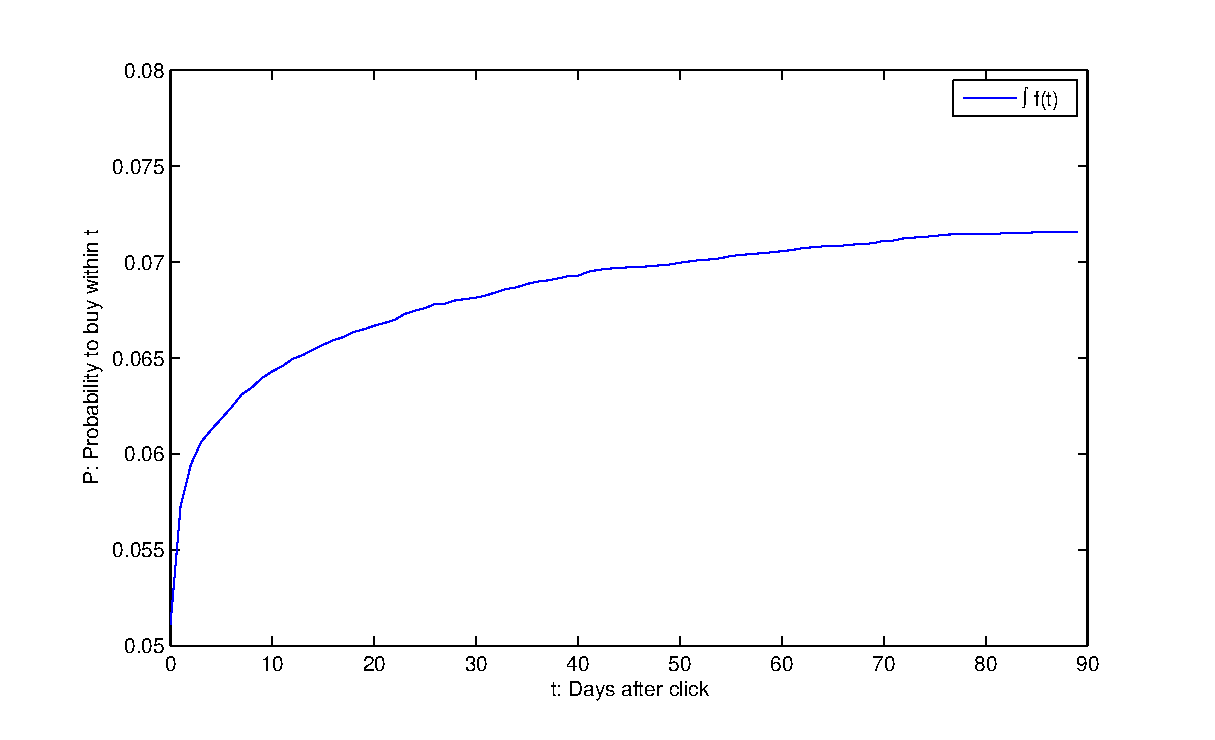
\includegraphics[width=\linewidth]{./click_curve.eps}
\caption{Integrated Transaction Probability for Click Behavior}
\label{fig:click-curve}
\end{figure}


\subsection{Item Similarity}


Similarity between items are usually computed in the space of $users$, treating each item as a vector. Classes of similarity methods includes \emph{cosine similarity}, \emph{adjusted cosine similarity} and \emph{Pearson correlation coefficient}, all of which are implemented.

~

Cosine Similarity

\begin{equation}
sim(\vec{u},\vec{v}) = \cos(\vec{u},\vec{v}) = \frac{\vec{u}\cdot \vec{v}}{||\vec{u}|| \cdot ||\vec{v}||}
\end{equation}

tends to be high when if each user who purchases u also purchases v as well. At the same time, frequently purchased items are de-emphasized by the denominator.

~

Adjusted Similarity\cite{sarwar2001item}

\begin{equation}
sim(i,j) = \frac{\sum_{u \in U}(R_{u,i} - \overline{R_u})(R_{u,j} - \overline{R_u})}{\sqrt{\sum_{u \in U}(R_{u,i} - \overline{R_u})^2}\sqrt{\sum_{u \in U}(R_{u,j} - \overline{R_u})^2}}
\end{equation}

takes different rating scales between users are taken into account.

~

Pearson Correlation Coefficient\cite{sarwar2001item}

\begin{equation}
sim(i,j) = \frac{\sum_{u \in U}(R_{u,i} - \overline{R_i})(R_{u,j} - \overline{R_j})}{\sqrt{\sum_{u \in U}(R_{u,i} - \overline{R_i})^2}\sqrt{\sum_{u \in U}(R_{u,j} - \overline{R_j})^2}}
\end{equation}

is a measure of the linear dependence between two variables. Here we need isolate co-rated cases in advance.


\subsection{Prediction}

$P_{u,i}$ is computed by summing the similarities between item $i$ and items in user $u$'s basket:

\begin{equation}
P_{u,i} = \sum_{Rank(s_{i,j})\geq k} s_{i,j} \cdot R_{u,j}
\end{equation}

This summing approach often results in high predictions when infrequently purchased items have a moderate overlap. One solution is to treat recommendations from each item $j$ as independent events.  Thus:

\begin{equation}
P_{u,i} = 1 - \prod_{Rank(s_{i,j})\geq k} (1 - s_{i,j} \cdot R_{u,j})
\end{equation}

Only if all recommendation fails, $R_{u,i} = 0$.

~

Another solution is similarity normalization. We can normalize the k similarities so that they add-up to 1.
\begin{equation}
s'_{i,j} = \frac{s_{i,j} }{ \sum_{Rank(s_{i,l})\geq k} s_{i,l} }
\end{equation}

~

At the same time, for users who purchases a lot, each item reflects his appetite less. We can normalize $R$ before doing prediction, which is called \emph{Row Normalization}.


\subsection{Post Procession}

In the case of ecommerce transaction, if user $u$ once purchased item $i$, whether he'll purchase another depends on the lifetime of item $i$:

\begin{equation}
\tau_i \approx \frac{\sum_{u \in U, R_{u,i}=1} R_{u,i}}{\sum_{u \in U, R_{u,i}=1}1 \cdot TimeSpan}
\end{equation}

Thus the modified $P_{u,i}$ should be:

\begin{equation}
    P'_{u,i} = \left\{ 
    \begin{array}{l l}
    P_{u,i} & \quad \text{if $R_{u,i} \neq 1$ }\\
    \frac{Timespan_{prediction}}{\tau_i} \cdot P_{u,i} & \quad \text{otherwise}
    \end{array} \right.
\end{equation}


\section{Evaluation}


The quality of recommender system is measured by $recall$ and $precision$.  $recall$ is the percentage of hits in the test set.  $precision$ is the percentage of hits in the prediction set.  $F1$ is used to combine these two parameters:
\begin{equation}
F1 = \frac{2}{1/recall + 1/precision}
\end{equation}


\subsection{DataSet}

In order to measure recommendation quality, we split the dataset into train set and test set, as in Table \ref{tab:train-test}.

\begin{table}[!h]
\centering
\begin{tabular}{ | l | l | l | }
\hline
~           & Train Set & Test Set \\ \hline
Begin Date  & 15th April    & 15th July  \\ \hline
End Date    & 14th July     & 14th August  \\ \hline
No. Transaction    & 4971   & 2013    \\ \hline
\end{tabular}
\caption{Train and Test Dataset}
\label{tab:train-test}
\end{table}


\subsection{Pre and Post Processing}

The effect of \emph{behavior statistic} is shown in Figure \ref{pic:pre}, compared to neglecting behaviors other than purchasement.

\begin{figure}[!h]
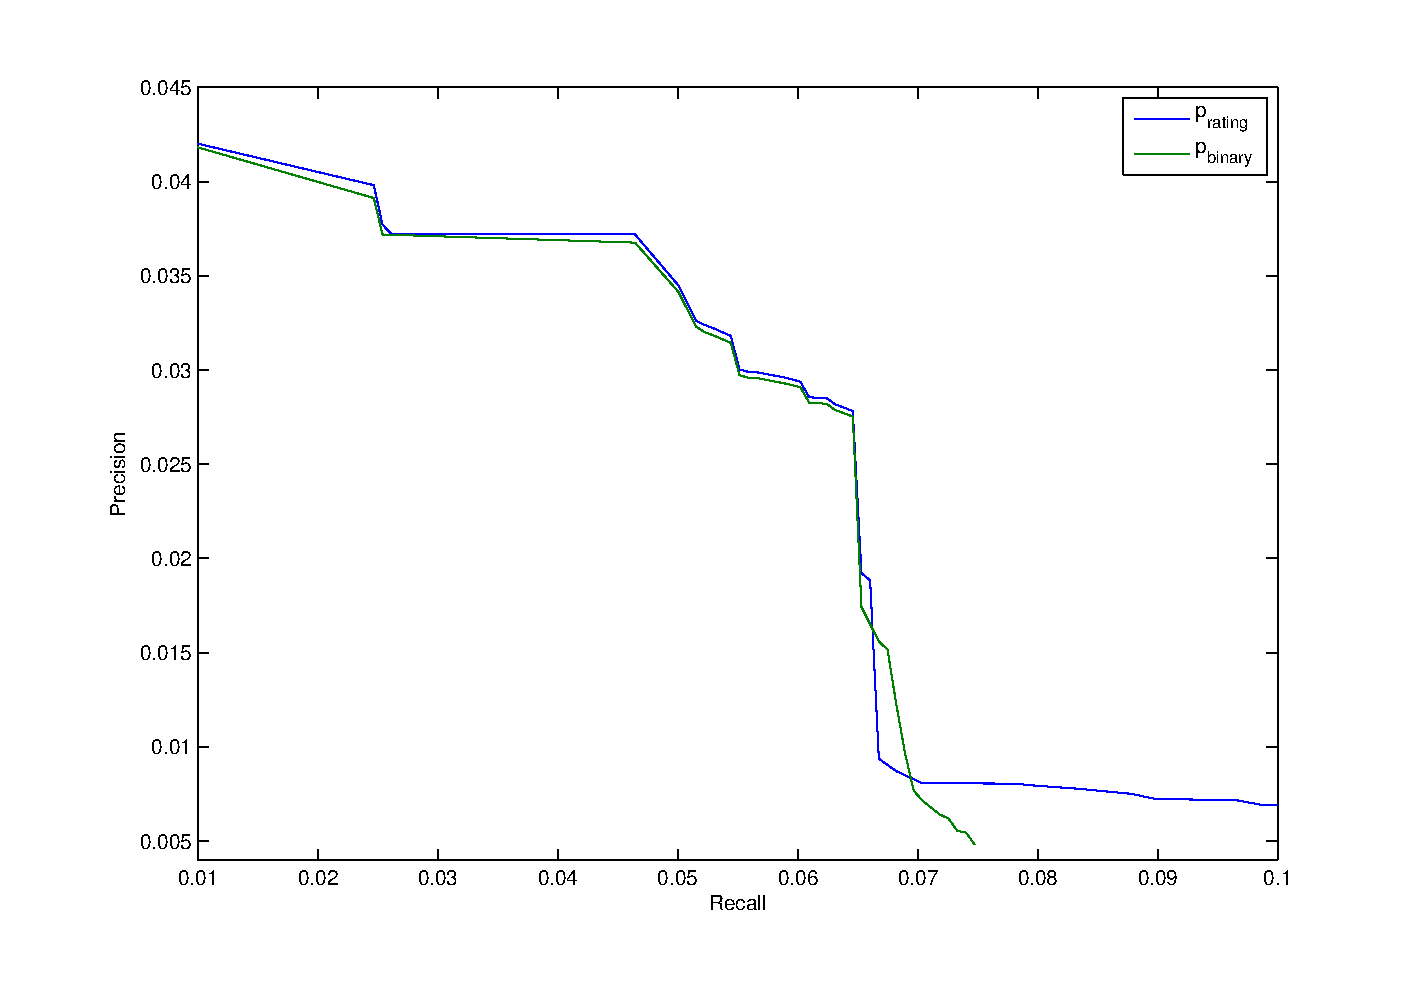
\includegraphics[width=\linewidth]{./rating.eps}
\includegraphics[width=\linewidth]{./rating_f1.eps}
\caption{The Effect of Behavior Statistic}
\label{pic:pre}
\end{figure}

~

The effect of \emph{post-processing} is shown in Figure \ref{pic:post}. The precision is better between 0.01 and 0.03. The smaller minimum F1 implies that post processing needs to be conducted judiciously.

\begin{figure}[!h]
\includegraphics[width=\linewidth]{./post-proc.eps}
\includegraphics[width=\linewidth]{./post-proc_f1.eps}
\caption{The Effect of Post Processing}
\label{pic:post}
\end{figure}


\subsection{Similarity Method Comparison}

Figure \ref{pic:simcomp} shows the results of \emph{correlation} and \emph{cosine} are approximate, while \emph{adjusted cosine} is bad. It is because adjusted cosine removes the difference in rating scales, which means positive rating could contain negative information. While for ecommerce data, positive rating is always positive.

\begin{figure}[!h]
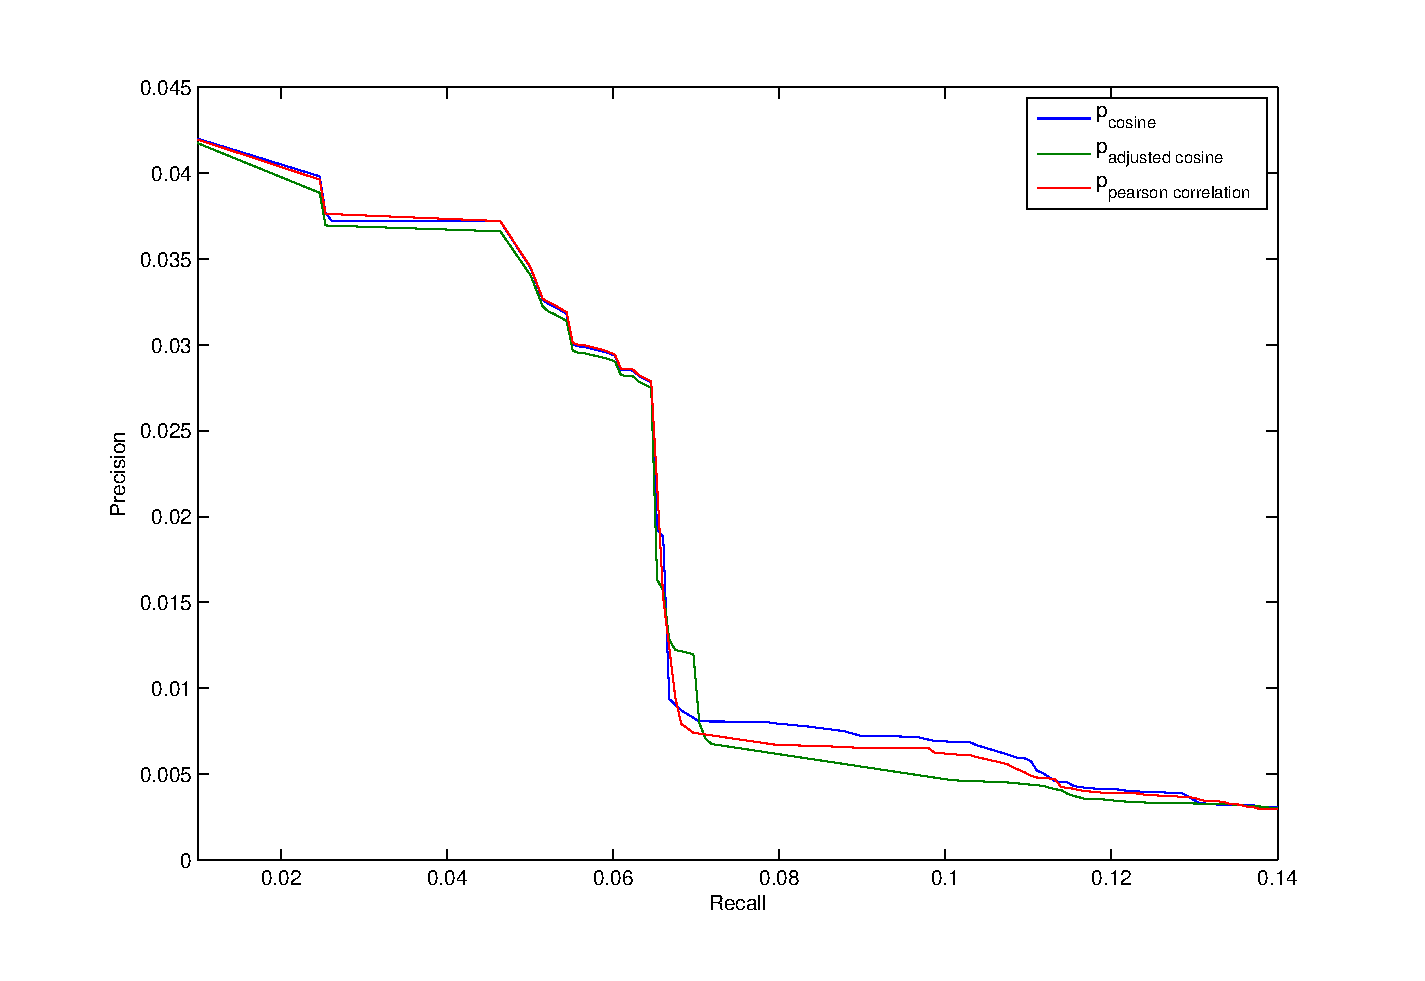
\includegraphics[width=\linewidth]{./sim_compare.eps}
\includegraphics[width=\linewidth]{./sim_compare_f1.eps}
\caption{Comparison Between Different Similarity Methods}
\label{pic:simcomp}
\end{figure}


\subsection{Summing and Normalization}

Apparently, summing appoach using conditional probability is better, as Figure \ref{pic:sumcomp} shows.

\begin{figure}[!h]
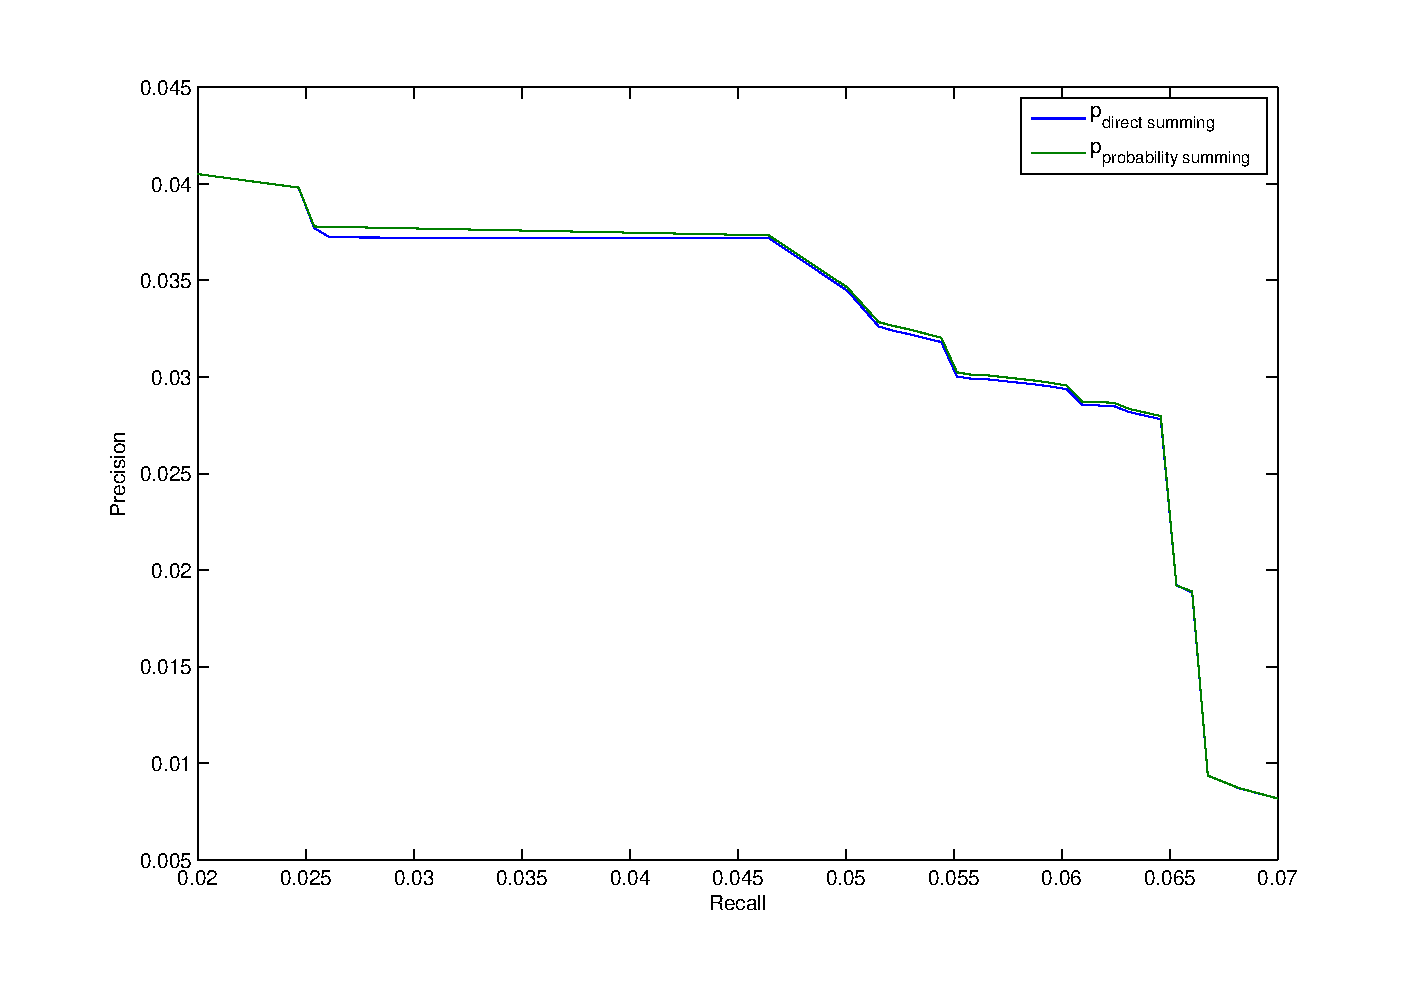
\includegraphics[width=\linewidth]{./summing_compare.eps}
\includegraphics[width=\linewidth]{./summing_compare_f1.eps}
\caption{Comparison Between Direct Summing and Probability Summing}
\label{pic:sumcomp}
\end{figure}

~

Figure \ref{pic:simnorm} shows \emph{similarity normalization} does no good in prediction, the primary reason is the dataset is so small that many items do not have $k$ neighbors. The sparse item will divide a smaller denominator, rather than larger(expected).

\begin{figure}[!h]
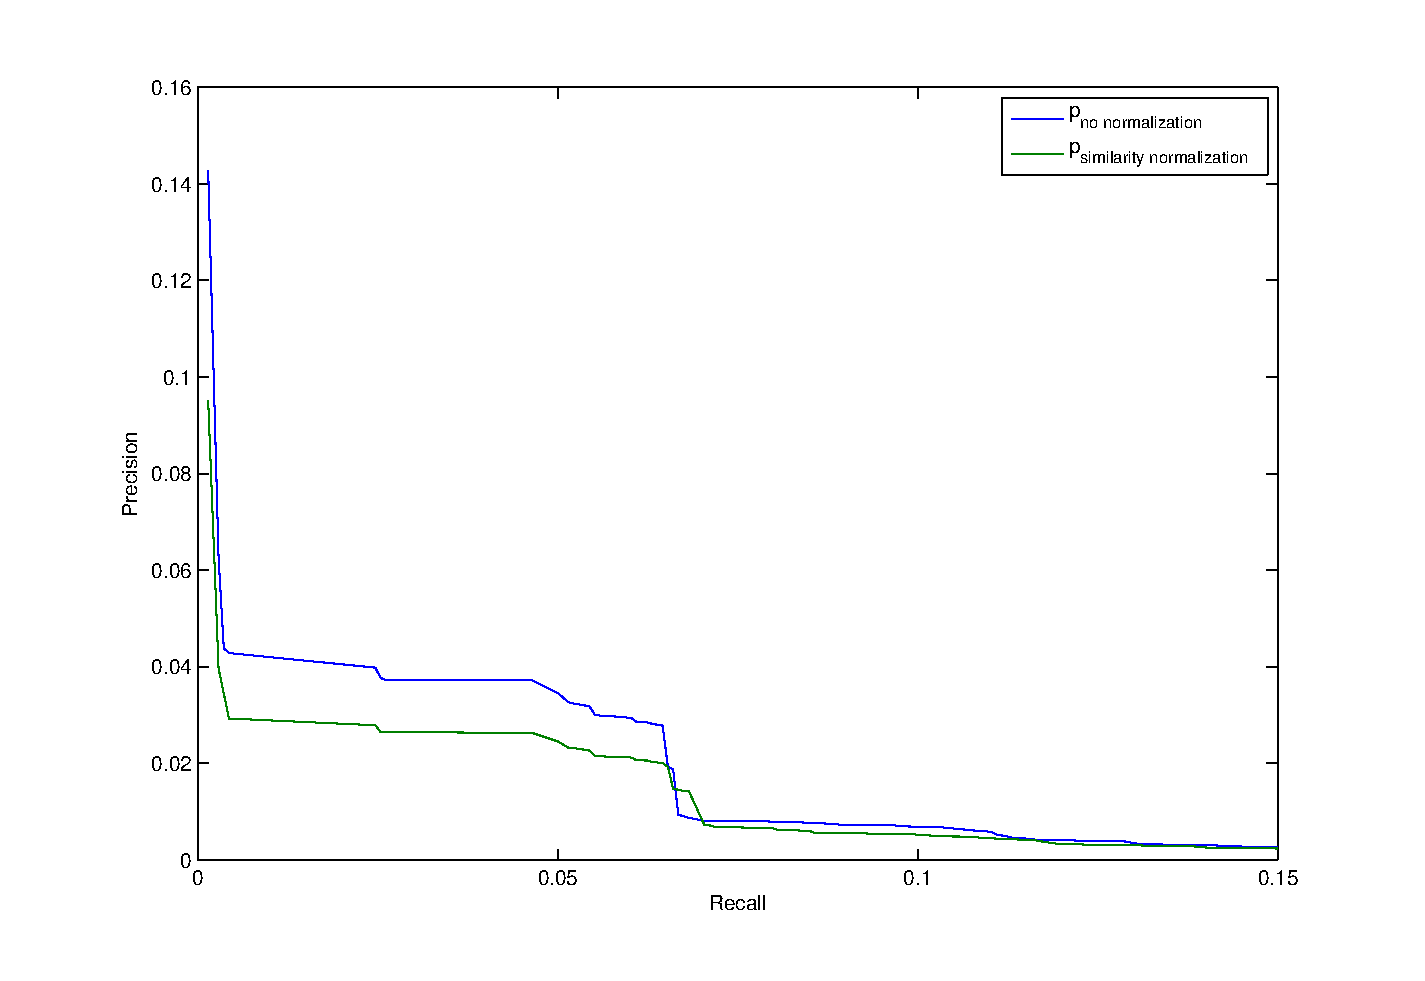
\includegraphics[width=\linewidth]{./sim_norm.eps}
\includegraphics[width=\linewidth]{./sim_norm_f1.eps}
\caption{Effect of Similarity Normalization}
\label{pic:simnorm}
\end{figure}

~

Figure \ref{pic:rownorm} shows \emph{row normalization} does no good. The side-effect of row normalization is normalized purchasing power for each user, while users who have purchased alot certainly will purchase a lot. Only in the case for Top-N Recommendation, in which we only recommend N item for each user. Normalizing purchasing power has no side-effect then.\cite{deshpande2004item}

\begin{figure}[!h]
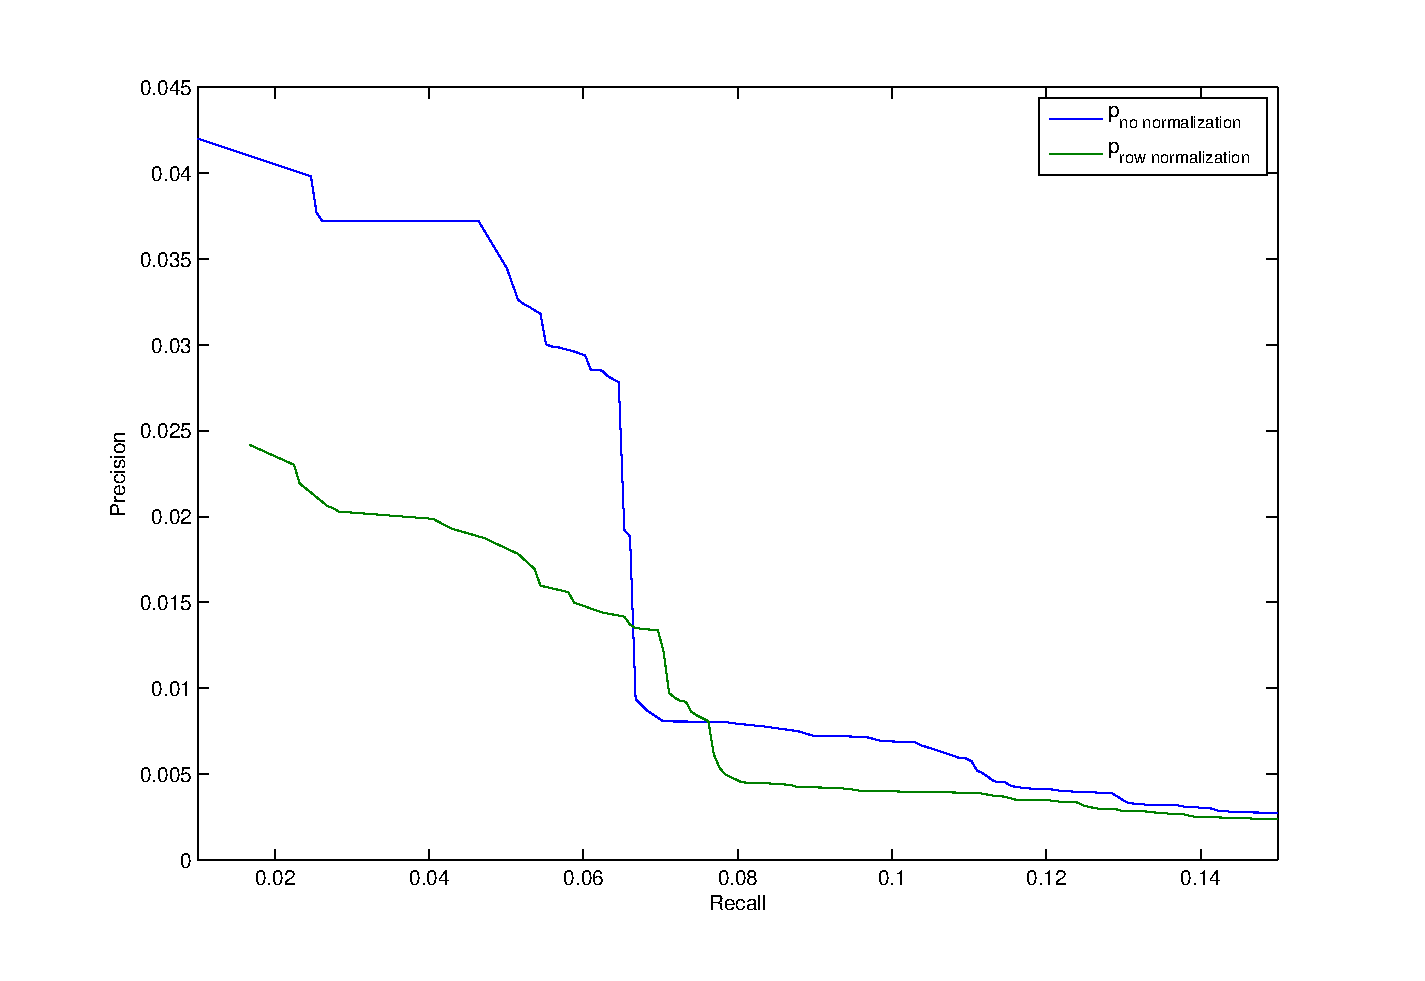
\includegraphics[width=\linewidth]{./row_norm.eps}
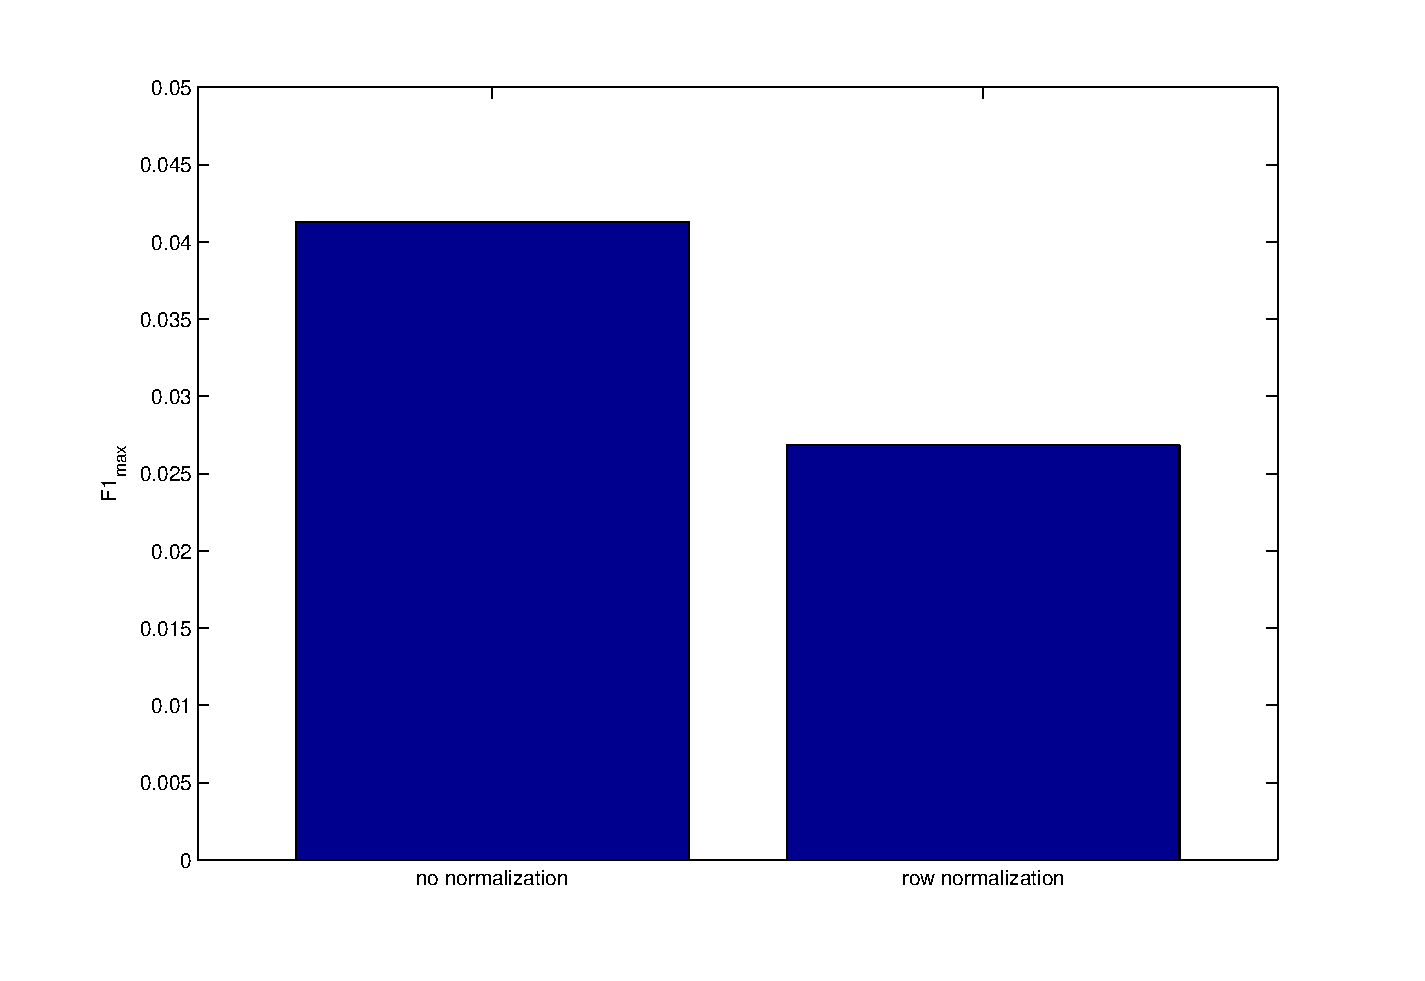
\includegraphics[width=\linewidth]{./row_norm_f1.eps}
\caption{Effect of Row Normalization}
\label{pic:rownorm}
\end{figure}


\subsection{Comparison with User-based CF}

Figure \ref{pic:usercomp} compares item-based CF with user-based CF. Almost no difference appears, while item-based CF is faster in realtime recommendation.

\begin{figure}[!h]
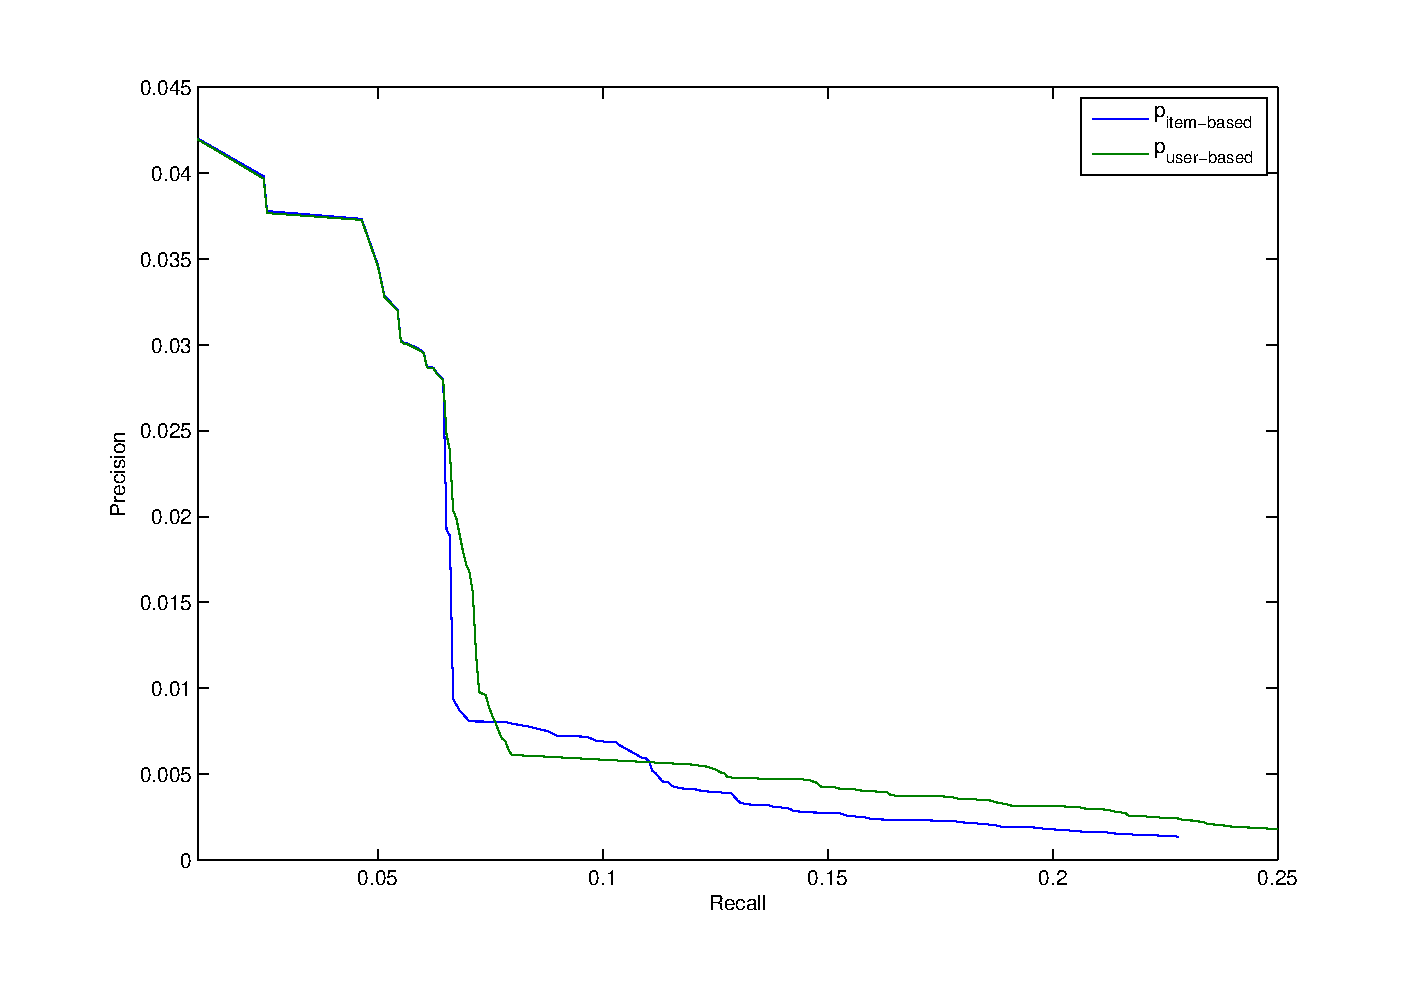
\includegraphics[width=\linewidth]{./base.eps}
\includegraphics[width=\linewidth]{./base_f1.eps}
\caption{Comparison Between Different Similarity Methods}
\label{pic:usercomp}
\end{figure}


\clearpage

\bibliographystyle{abbrv}\bibliography{doc.bib}

\end{document}
